\chapter{Bancos de dados}

\pagestyle{fancy}

Os bancos de dados são elementos fundamentais no ambiente computacional atual, com aplicação praticamente universal. Concebidos para um propósito geral, são úteis em qualquer disciplina que exija a gestão de dados — especialmente quando esses dados são volumosos.

No caso dos SIG, a quantidade de dados cresce constantemente, tanto em volume quanto em precisão. Além disso, há características específicas como múltiplos usos, necessidade de acesso eficiente e indexação, que recomendam o uso de bancos de dados e tecnologias próprias para sua gestão.

Entendemos por \emph{banco de dados} um \textbf{conjunto de dados estruturado e armazenado sistematicamente}, com o objetivo de facilitar seu uso posterior. A chave está na \textbf{estrutura} e \textbf{sistematização}, que tornam o banco de dados superior a uma simples coleção desorganizada de arquivos.

As vantagens diretas do uso de um banco de dados incluem:

\begin{itemize}
	\item \textbf{Maior independência}: os dados são independentes das aplicações e dos usuários.
	\item \textbf{Maior disponibilidade}: acesso facilitado a partir de diferentes sistemas e locais.
	\item \textbf{Maior segurança}: replicação e sincronização de dados mais confiáveis.
	\item \textbf{Menor redundância}: menos dados repetidos, maior rapidez.
	\item \textbf{Maior eficiência na entrada e codificação de dados}.
\end{itemize}

Isso se reflete diretamente nos resultados:

\begin{itemize}
	\item \textbf{Maior coerência}: melhor gestão → melhor qualidade dos dados.
	\item \textbf{Maior eficiência}: acesso rápido aos dados.
	\item \textbf{Maior valor informativo}: facilita a extração de informação relevante.
\end{itemize}

Para os usuários:

\begin{itemize}
	\item \textbf{Facilidade de acesso}: basta saber utilizar os dados, não gerenciá-los.
	\item \textbf{Reutilização de dados}: maior compartilhamento.
\end{itemize}

Resumidamente, a principal qualidade de um banco de dados é a \textbf{centralização} dos dados — o que melhora o gerenciamento, a estrutura e o acesso.

\section{Bancos de dados relacionais}

O modelo mais comum, tanto em SIG quanto em outras áreas, é o de \textbf{bancos de dados relacionais}, baseado em \textbf{tabelas}.

Cada tabela (ou \textbf{relação}) possui:

\begin{itemize}
 \item \textbf{Registros} (linhas)
 \item \textbf{Campos} (colunas)
\end{itemize}

Cada linha, chamada de \textbf{tupla}, representa uma entidade com atributos distintos.

Um banco de dados geralmente contém múltiplas tabelas interligadas. Para isso, utilizamos os \textbf{atributos-chave}, que são \textbf{únicos e invariáveis} para cada entidade (ex: número de CPF).

Em dados espaciais, a \textbf{geometria} pode ser usada como chave.

Relações entre tabelas podem ser:

\begin{itemize}
 \item \textbf{Um para um}
 \item \textbf{Um para muitos}
 \item \textbf{Muitos para muitos}
\end{itemize}

Exemplo: uma pessoa pode morar em uma cidade, mas uma cidade pode ter muitas pessoas.

\section{Sistemas gerenciadores de banco de dados (SGBD)}

O SGBD (ou DBMS — \emph{Database Management System}) é o \textbf{intermediário entre os dados e os aplicativos}, como o SIG.

Funções do SGBD:

\begin{itemize}
	\item \textbf{Acesso transparente}: o SGBD interpreta e executa consultas.
	\item \textbf{Proteção de dados}: controle de acesso e segurança.
	\item \textbf{Eficiência}: gerencia grandes volumes e acessos simultâneos.
	\item \textbf{Transações}: garante que as alterações sejam consistentes (\textbf{SGBD transacional}).
\end{itemize}

O principal \textbf{linguagem de consulta} é o \textbf{SQL} (Standard Query Language).

\subsection{Bancos de dados espaciais}

Para um banco de dados ser considerado \textbf{espacial}, ele precisa armazenar e entender dados espaciais nativamente.

\begin{itemize}
\item As geometrias são armazenadas diretamente como atributos.
\item O SGBD deve interpretar esses dados e responder a consultas espaciais.
\end{itemize}

Esse armazenamento é chamado de \textbf{transparente}. No armazenamento \textbf{opaco}, os dados são armazenados, mas não compreendidos.

Bases espaciais trabalham principalmente com \textbf{dados vetoriais}. A parte temática é armazenada como em qualquer banco relacional.

Também é necessário um \textbf{linguagem de consulta espacial}, com operadores próprios para lidar com relações espaciais.

\section{Consultas}

Consultas permitem "perguntar" algo aos dados — por exemplo: \emph{Quais rios passam por tal estado?}

Elas podem ser:

\begin{itemize}
 \item \textbf{Temáticas}: usam apenas os atributos.
 \item \textbf{Espaciais}: usam apenas a geometria.
 \item \textbf{Espacio-temáticas}: combinam ambos.
\end{itemize}

Exemplo visual: seleção por área retangular (Figura~\ref{Fig:Seleccion}).

\begin{figure}[!hbt]   
\centering
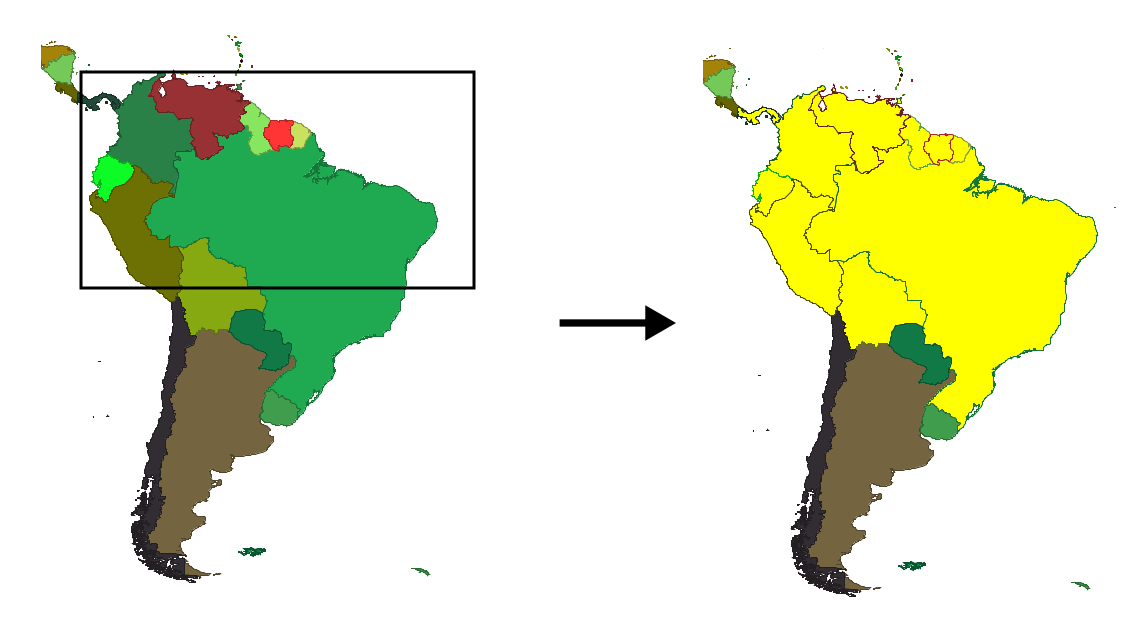
\includegraphics[width=\textwidth]{Bases_dados/Seleccion_rectangulo.png}
\caption{\small Consulta gráfica por seleção. Entidades dentro do retângulo são selecionadas.}
\label{Fig:Seleccion} 
\end{figure}

Exemplos de consultas temáticas:

\begin{itemize}
 \item Países com PIB maior que o do Brasil.
 \item Países com mais de 200 milhões de habitantes.
\end{itemize}

Consultas podem ser combinadas com \textbf{operadores booleanos}:

\begin{itemize}
 \item Países da zona do euro \emph{e} com mais de 40 milhões de habitantes.
 \item Países de língua inglesa \emph{e} com crescimento populacional.
\end{itemize}

Consultas espaciais:

\begin{itemize}
 \item Quais países fazem fronteira com a Argentina?
 \item Quantos países estão inteiramente no hemisfério sul?
 \item Quais países estão a menos de 2000 km do Brasil?
\end{itemize}

Consultas espacio-temáticas:

\begin{itemize}
 \item Países do hemisfério norte com densidade populacional maior que a do Peru.
 \item Países com mais de 10 milhões de habitantes a menos de 1000 km da Rússia.
\end{itemize}

Consultas entre \textbf{múltiplas camadas} também são possíveis. Exemplo: unir cidades com os países onde estão localizadas (por nome ou por localização espacial — \textbf{junção espacial}).

\subsection{Índices espaciais}

Consultas diretas exigem varrer toda a base — o que é ineficiente.

\textbf{Índices} permitem localizar registros rapidamente, sem precisar varrer tudo.

\textbf{Índices espaciais} funcionam de forma semelhante. Eles ajudam o SIG a identificar onde buscar, reduzindo operações desnecessárias.

Exemplo: para saber quais países estão a menos de 3000 km da Espanha, descartamos automaticamente as Américas. Isso é uma forma intuitiva de índice espacial.

O SGBD pode armazenar esses índices junto com os dados ou em arquivos adicionais.

\pagestyle{empty}
